
\eat{
\begin{figure}[tb!]
%\vspace{-2ex}
\begin{center}
%\hspace{10ex}
\subfigure[{\scriptsize TWPageRank (batch vs. increm.)}]{\label{fig-aminer-time2}
\includegraphics[scale=0.38]{./exp/MAG_time_twpr.eps}}
%\quad\quad
\hspace{-0.5ex}
\subfigure[{\scriptsize Comparison of ranking algorithms}]{\label{fig-aminer-time1}
\includegraphics[scale=0.38]{./exp/MAG_time.eps}}
\end{center}
\vspace{-5ex}
\caption{\small Results of efficiency on \aminer}
\label{fig-aminer-time}
\vspace{-3ex}
\end{figure}
%%%%%%%%%%%%%%%%%%%%%
\begin{figure}[tb!]
%\vspace{-2ex}
\begin{center}
%\hspace{10ex}
\subfigure[{\scriptsize TWPageRank (batch vs. increm.)}]{\label{fig-aminer-time-sigma}
\includegraphics[scale=0.38]{./exp/MAG_time_twpr.eps}}
%\quad\quad
\hspace{-0.5ex}
\subfigure[{\scriptsize Comparison of ranking algorithms}]{\label{fig-mag-time-sigma}
\includegraphics[scale=0.38]{./exp/MAG_time.eps}}
\end{center}
\vspace{-5ex}
\caption{\small Results of efficiency on \aminer}
\label{fig-time-sigma}
\vspace{-3ex}
\end{figure}
}


\begin{figure*}[tb!]
\vspace{-2ex}
\begin{minipage}[t]{0.5\textwidth}
\begin{center}
\subfigure[{\scriptsize TWPageRank (batch vs. inc.)}]{\label{fig-aminer-time2}
\includegraphics[scale=0.38]{./exp/AMiner_time_twpr.eps}}
%\quad\quad
\hspace{-0.5ex}
\subfigure[{\scriptsize Comparison of ranking algorithms}]{\label{fig-aminer-time1}
\includegraphics[scale=0.38]{./exp/AMiner_time.eps}}
\end{center}
\vspace{-5ex}
\caption{\small Efficiency tests on \aminer}
\label{fig-aminer-time}
\end{minipage}
\hspace{-2ex}
\begin{minipage}[t]{0.5\textwidth}
\begin{center}
\subfigure[{\scriptsize \aminer}]{\label{fig-aminer-time-sigma}
\includegraphics[scale=0.38]{./exp/AMiner_sigma_time.eps}}
%\quad\quad
\hspace{-0.5ex}
\subfigure[{\scriptsize \magdata}]{\label{fig-mag-time-sigma}
\includegraphics[scale=0.38]{./exp/MAG_sigma_time.eps}}
\end{center}
\vspace{-5ex}
\caption{\small Efficiency tests: varying $\sigma$}
\label{fig-time-sigma}
\end{minipage}
\vspace{-1ex}
\end{figure*}



\vspace{-1ex}
\section*{APPENDIX A: Further Experiments}
\label{sec-exp-app}


\subsection*{1. Exp-3: Efficiency}

In the third of tests, we evaluated the efficiency of our batch and incremental algorithms.
We compared our algorithms with \powensemble, \powtwprdag, and \powtwprscc, as well as baselines \futurerank and \hhgrank.
The results on \aminer are reported in Fig.~\ref{fig-aminer-time}.

Similar to the results on \magdata, when varying $Y_s$, the running time of all algorithms increases with the increment of $Y_s$, and the incremental algorithms
consistently run faster than other counterparts on \aminer.
For TWPageRank, algorithms \twprdag and \twprscc
%, which compute TWPageRank on citation and venue graphs,
are 1.8 and 2.1 times faster than \powtwprdag and \powtwprscc on average, respectively. And algorithms \inctwprdag and \inctwprscc further improve the efficiency  by 31\% and 35\% on average, compared with \twprdag and \twprscc, respectively.
%By these, we have also experimentally shown that the efficiency improvement of \inctwprscc, even it does not change the time complexity.
%
For scholarly article ranking, algorithm \batensemble is on average (1.1, 2.0, 181) times faster than (\powensemble, \futurerank, \hhgrank), respectively.
And algorithm \incensemble further improves the efficiency by 27\% on average, compared with \batensemble.
%When varying $Y_s$, the running time for TWPageRank computation on the citation and venue ensemble increase with the increment of $Y_s$.


\newcommand{\graphscaleexpapp}{0.262}
\newcommand{\graphmarginexpapp}{-2ex}
%%% all in 1 Figure
\begin{figure*}[tb!]
%\vspace{-2ex}
\begin{center}
%\hspace{-10ex}
\subfigure[{\scriptsize \aan}]{\label{fig-aan-ab-recom}
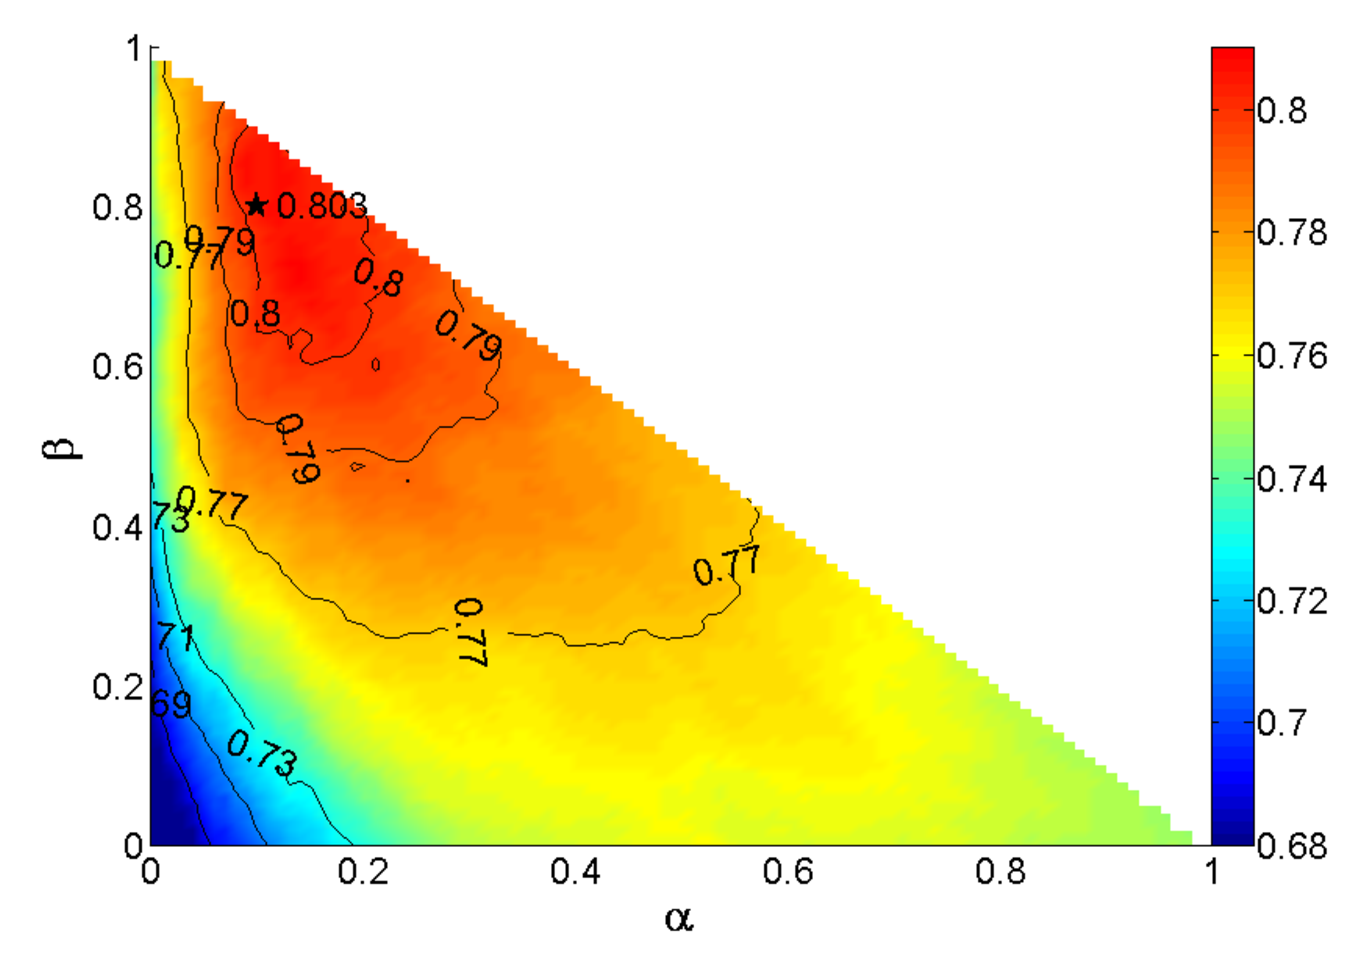
\includegraphics[scale=\graphscaleexpapp]{./exp/AAN-para-recm.eps}}
%\quad\quad
\hspace{\graphmarginexpapp}
\subfigure[{\scriptsize \aminer}]{\label{fig-aminer-ab-recom}
\includegraphics[scale=\graphscaleexpapp]{./exp/AMiner-para-recm.eps}}
%\quad\quad
\hspace{\graphmarginexpapp}
\subfigure[{\scriptsize \magdata}]{\label{fig-mag-ab-recom}
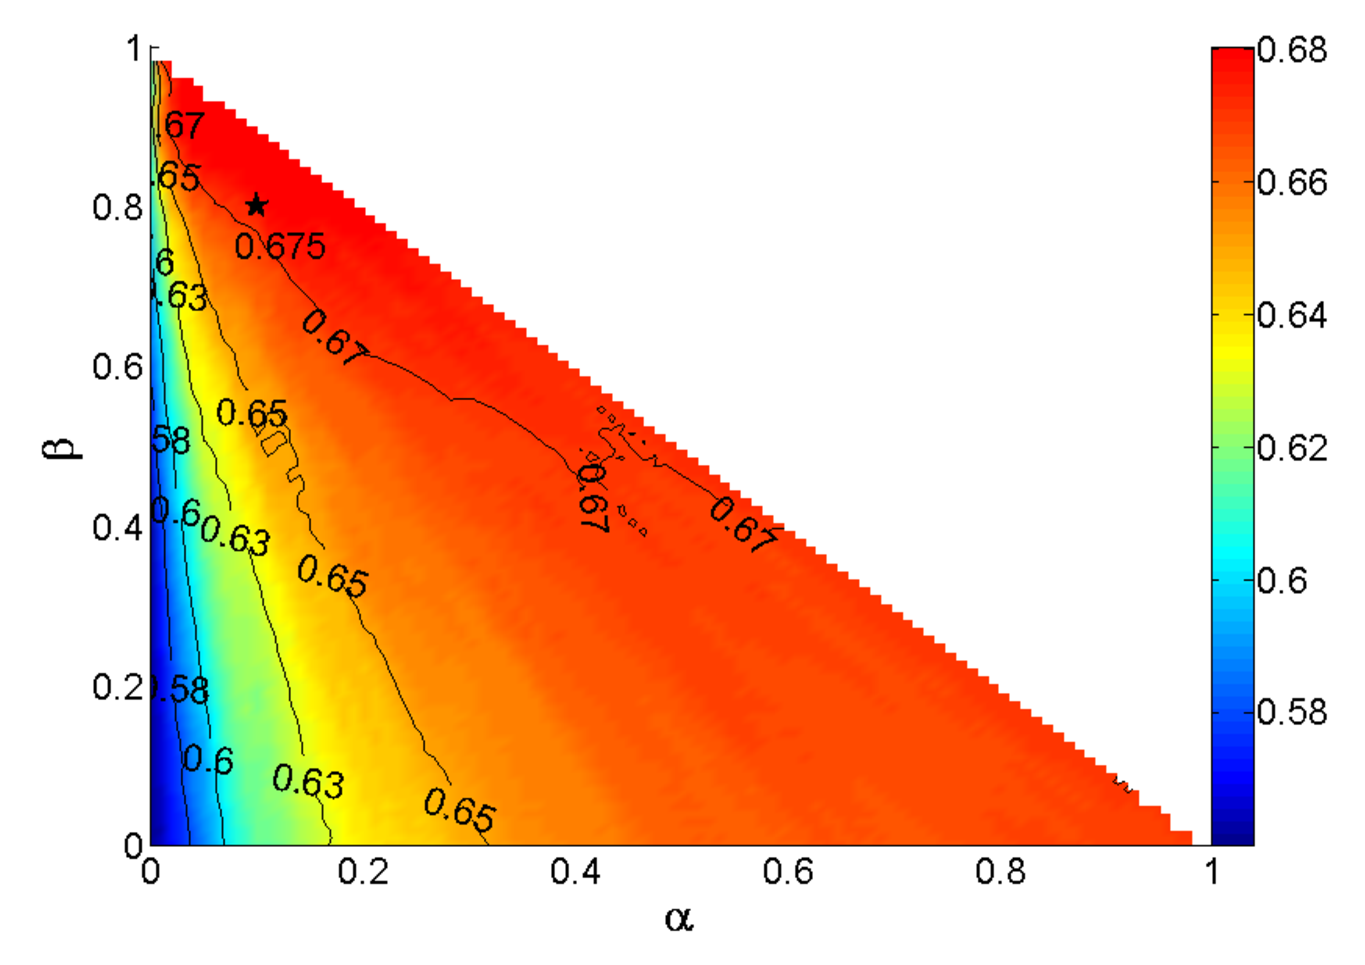
\includegraphics[scale=\graphscaleexpapp]{./exp/MAG-para-recm.eps}}
\\ %%%%%%%%%%%%%%%%%%%%%%%%%%%%%%%%%%%%%%
\vspace{-3ex}
%\hspace{-10ex}
\subfigure[{\scriptsize \aan}]{\label{fig-aan-ab-fcita}
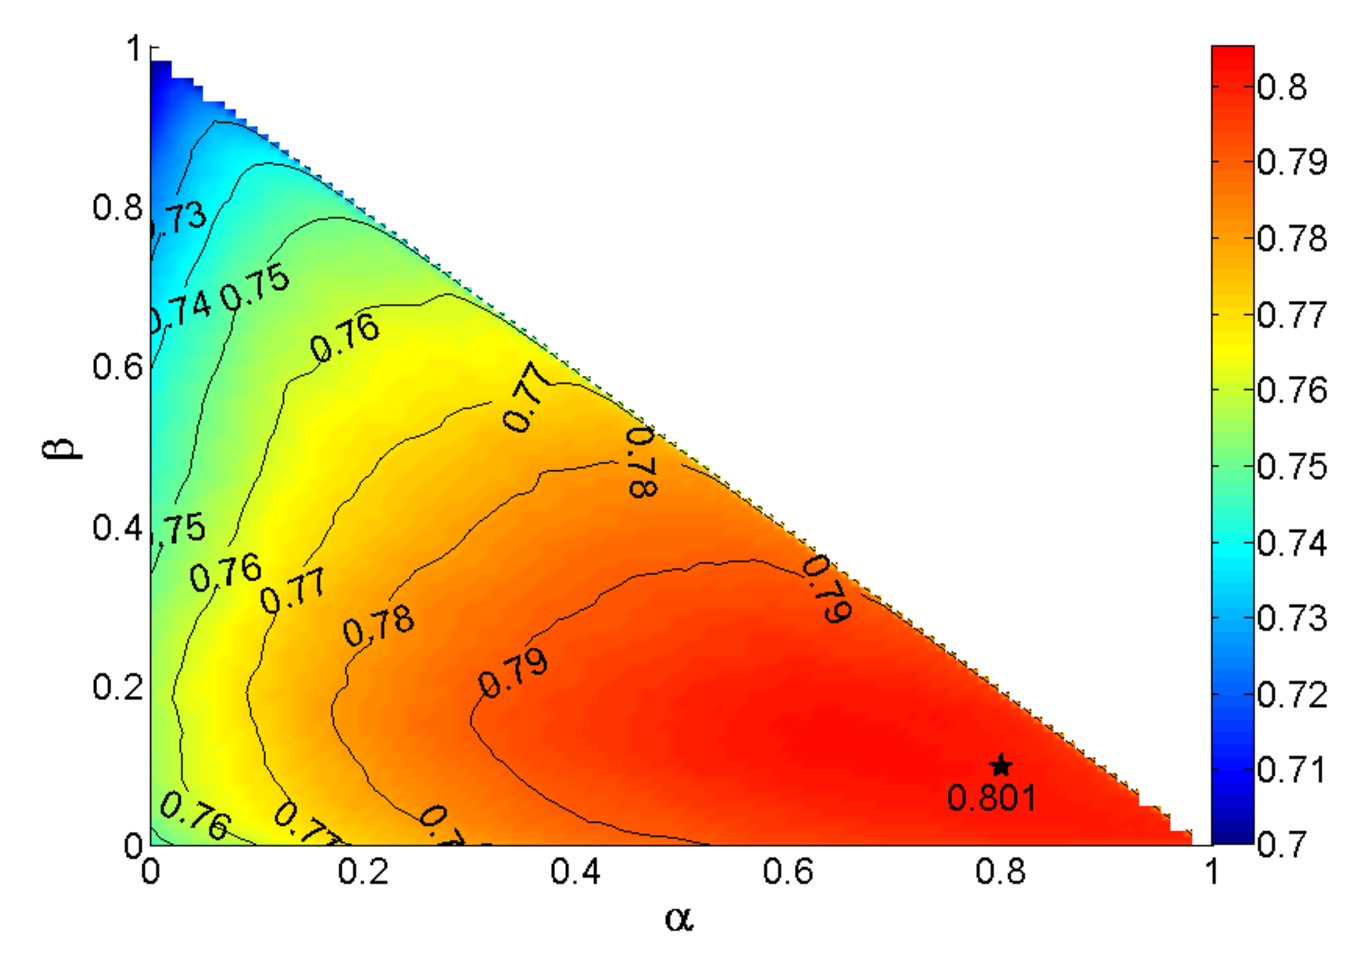
\includegraphics[scale=\graphscaleexpapp]{./exp/AAN-para-fcita.eps}}
%\quad\quad
\hspace{\graphmarginexpapp}
\subfigure[{\scriptsize \aminer}]{\label{fig-aminer-ab-fcita}
\includegraphics[scale=\graphscaleexpapp]{./exp/AMiner-para-fcita.eps}}
%\quad\quad
\hspace{\graphmarginexpapp}
\subfigure[{\scriptsize \magdata}]{\label{fig-mag-ab-fcita}
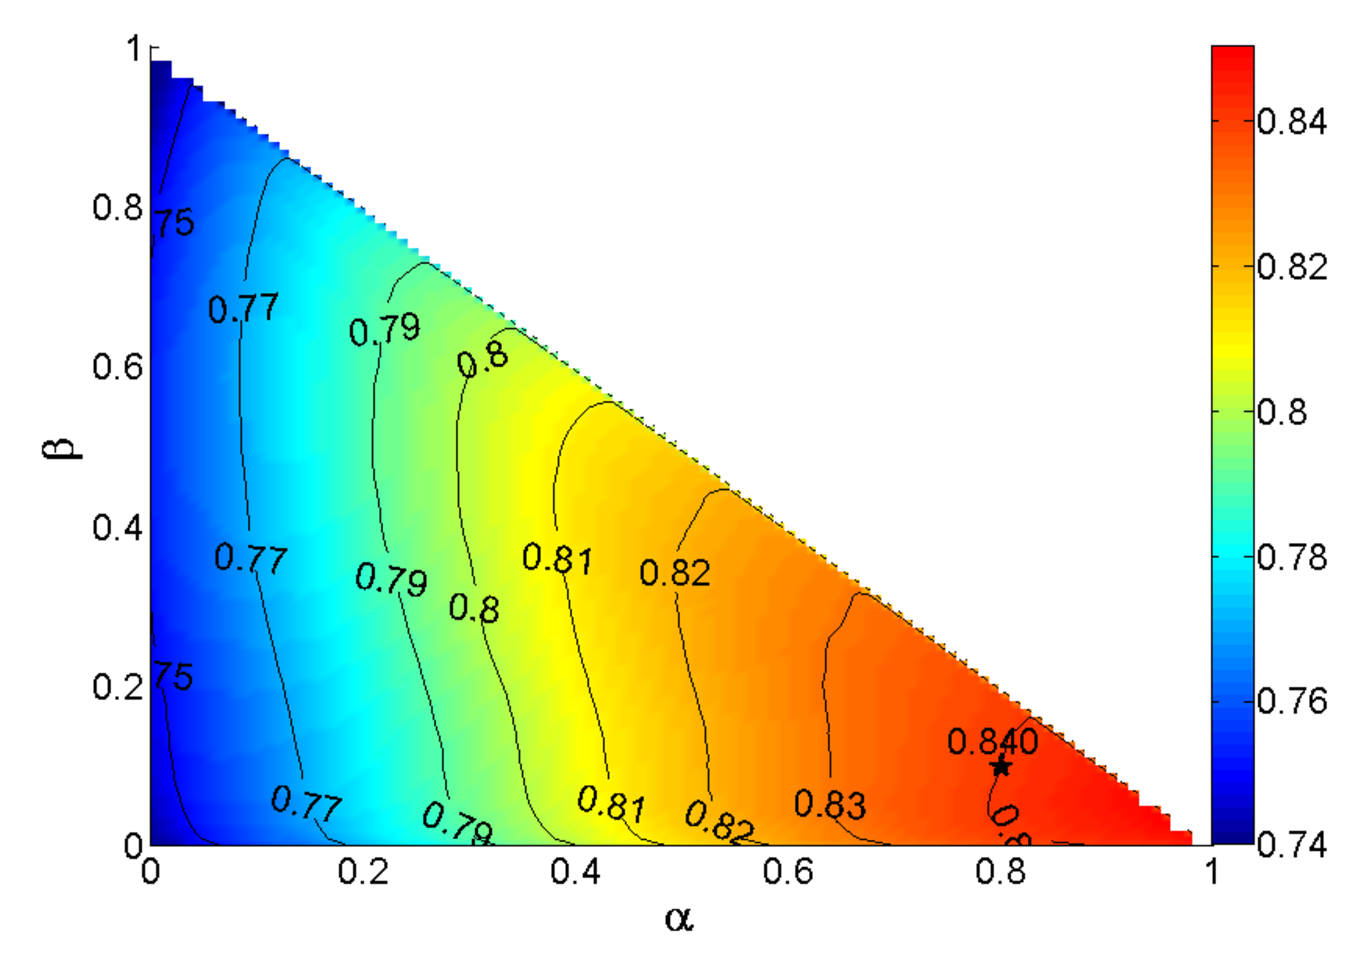
\includegraphics[scale=\graphscaleexpapp]{./exp/MAG-para-fcita.eps}}
\end{center}
\vspace{-5ex}
\caption{\small Accuracy tests on \recom ((a)--(c)) and \fcita ((d)--(f)): varying parameters $\alpha$ and $\beta$}
\label{fig-ab}
\vspace{-3ex}
\end{figure*}
%%%%%%%%%%%%%%%%%%%%%%%%%%%%%%%%%%%%%%

\subsection*{2. Detailed results of Exp-4} %$\alpha$ and $\beta$ (detailed)

We present detailed results of Exp-4, which are omitted earlier due to the space constraints, \ie the impacts of the time decaying factor $\sigma$  on efficiency  ({\em Exp-4.1}) and the impacts of parameters $\alpha$ and $\beta$ on effectiveness ({\em Exp-4.2}).

\etitle{Exp-4.1}. To evaluate the impacts of the time decaying factor $\sigma$, we varied $\sigma$ from -1.6 to -0.4, while fixed $Y_s$ to default values, $b=+\infty$ and $dif=1$. The efficiency results are reported in Fig.~\ref{fig-time-sigma}.
Note that the running time of algorithm \batensemble is different on \recom and \fcita because of the different splitting year $Y_s$.

When varying $\sigma$, the running time of \batensemble is almost stable on both \aminer and \magdata using \fcita and \recom. Indeed, the running time using (\fcita, \recom) only varies (1.4\%, 0.5\%) on \aminer, and (2.1\%, 2.2\%) on \magdata, on average, respectively.


\etitle{Exp-4.2}.
To evaluate the impacts of parameters $\alpha$ and $\beta$ on effectiveness, we varied $\alpha$ and $\beta$ at the granularity of 0.01, while fixed $Y_s$ to default values, $b=+\infty$, $Dif=1$ and $\sigma=-1.0$. The results are reported in Fig.~\ref{fig-ab}, where the parameters selected earlier and their corresponding \PairAcc are marked with $*$.

When varying $\alpha$ and $\beta$, the \PairAcc of \ensemblerank changes gently, as shown in Fig.~\ref{fig-ab}.
The optimal \PairAcc is obtained within a single region, rather than a complex collection of optimal regions.
%
Moreover, the \PairAcc keeps at a high level within a certain ($\alpha$, $\beta$) combination space around the optimal region.
For instance, consider a square of length 0.3, which covers 8.5\% of the parameter combination space. The fraction of parameters such that the \PairAcc is no worse than 1\% of the corresponding \PairAcc with marker $*$ is (73\%, 94\%) on \aan, (96\%, 87\%) on \aminer and (83\%, 95\%) on \magdata, using (\recom, \fcita), respectively.
%
Further, the optimal parameters on the same benchmarks are very similar for (\aan, \aminer and \magdata), indicating that the setting of $\alpha$ and $\beta$ can be easily transferred across different datasets.
To conclude, \ensemblerank is very robust to parameters $\alpha$ and $\beta$, and it is quite flexible for choosing proper values of parameters $\alpha$ and $\beta$.

%For instance, consider a square of length 0.3, which covers 8.5\% of all parameter combinations.
%The fraction of parameters such that the \PairAcc is no worse than 1\% of the corresponding \PairAcc reported earlier is (73\%, 94\%) on \aan, (96\%, 87\%) on \aminer and (83\%, 95\%) on \magdata, using (\recom, \fcita), respectively. (See \cite{ERank-full} for complete results.)

